\documentclass[12pt]{article}
\usepackage{graphicx}
\usepackage[a4paper, margin=1in]{geometry}
\usepackage{url}
\usepackage{amsmath}
\usepackage{hyperref}
\usepackage{float}
\usepackage{booktabs}
\usepackage{multirow}

\title{Segmenting Credit Card Users: \\ Leveraging the Power of Clustering through the KDD Process}
\date{\today}

\begin{document}

\maketitle

\begin{abstract}
In an era where personalization and tailored marketing strategies are paramount for businesses, understanding customer behaviors and segmenting them accordingly is of utmost importance. This research employs the Knowledge Discovery in Databases (KDD) process to delve into a dataset of credit card users, aiming to segment users based on their behavioral patterns. Through rigorous data processing, exploration, and clustering, distinct segments emerge, each offering unique insights and opportunities for targeted marketing strategies. The findings of this study serve as a foundation for businesses seeking to refine their customer engagement and marketing efforts.
\end{abstract}

\section{Introduction}

The digital age has ushered in an era where vast amounts of data are at the fingertips of organizations. For businesses, especially in the financial sector, this data is a goldmine, offering insights into customer behaviors, preferences, and patterns. Among the various data types, credit card transaction data is particularly intriguing, encapsulating a user's spending habits, preferences, and financial behaviors.

Segmenting users based on this data can unveil distinct groups with unique characteristics, enabling businesses to tailor their services, offers, and marketing strategies accordingly. This research navigates this segmentation journey, harnessing the power of the KDD process and clustering techniques.

\section{Data Understanding}

The dataset under scrutiny encapsulates the behaviors of 8950 active credit card users, spanning 18 behavioral variables. These variables range from basic metrics like balance and credit limit to more intricate ones like purchase frequency and cash advance transactions.

A cursory exploration of the dataset reveals:
\begin{itemize}
\item A diverse range of balances, with some users maintaining high balances and others minimal amounts.
\item Various purchasing behaviors, with certain users inclined towards one-off purchases and others towards installment-based ones.
\item Discrepancies in credit limits, indicating differing creditworthiness among users.
\item Missing data points in certain columns, necessitating preprocessing steps before deeper analysis.
\end{itemize}

\section{Data Preparation}

A rigorous data preparation phase was undertaken to ensure the dataset's suitability for clustering. This phase is pivotal in the KDD process as it sets the stage for effective data mining. Key steps included:

\begin{itemize}
    \item 
        \textbf{Missing Value Imputation:} Credit card data often contains missing values, either due to errors or omissions. The CREDIT\_LIMIT and MINIMUM\_PAYMENTS columns, which had missing values, were addressed by imputing the mean of the respective columns. This strategy ensured that the overall distribution of these columns remained unaffected, while providing a reasonable estimate for the missing values.
    \item 
        \textbf{Standardization:} Given the varying scales and units of the dataset's features, a standardization step was crucial. This ensured that each feature contributed equally to the clustering process, preventing any single feature from dominating the clustering due to its scale.

    \item 
        \textbf{Dimensionality Reduction:} With a multitude of features, reducing dimensionality can simplify the clustering process and make visualizations feasible. Employing Principal Component Analysis (PCA), the dataset's dimensionality was reduced, making it more manageable and visualization-friendly. The first two principal components, which captured a significant portion of the dataset's variance, were retained for subsequent steps.
    \end{itemize}

\section{Modeling}

The modeling phase is a pivotal step within the Knowledge Discovery in Databases (KDD) process. It entails the application of data mining algorithms to extract patterns or knowledge from the prepared dataset. The overarching goal of this phase was to segment credit card users based on their behavioral patterns.

\subsection{Optimal Cluster Determination}

Before diving into clustering, it's imperative to determine the optimal number of clusters. This ensures the granularity of segmentation is neither too broad nor too specific. 

The elbow method was employed for this purpose, a technique that identifies the number of clusters at which the reduction in within-cluster variance starts to show diminishing returns. 

\begin{figure}[H]
    \centering
    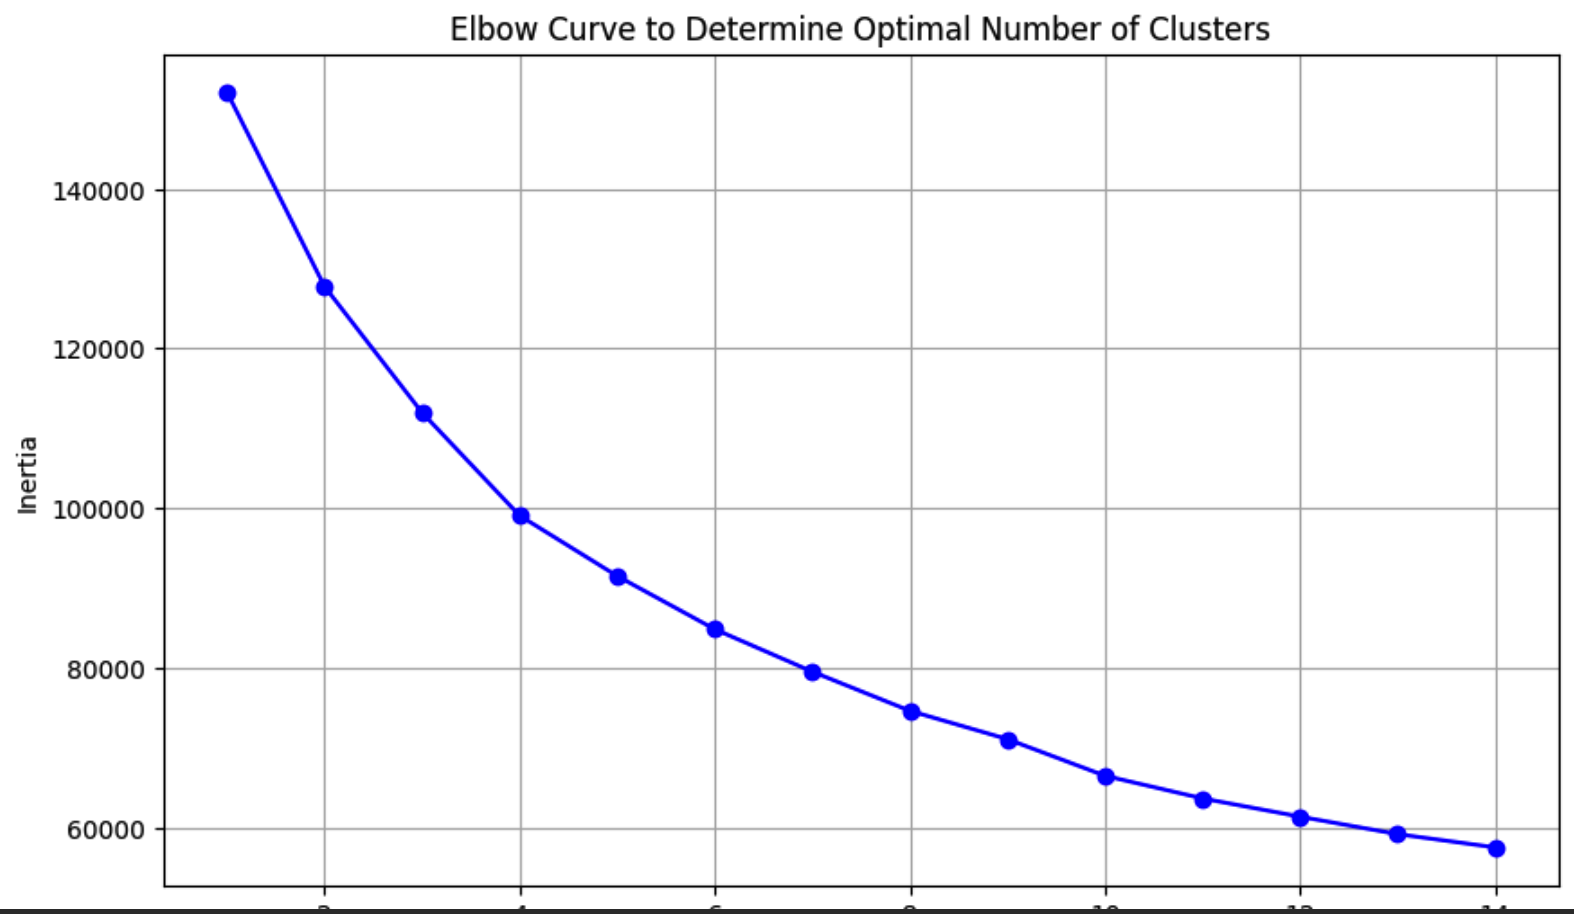
\includegraphics[width=0.7\linewidth]{elbow_plot.png}
    \caption{Elbow Plot for Determining Optimal Number of Clusters}
    \label{fig:elbow_plot}
\end{figure}

From the elbow plot, the inflection point around four clusters suggested that segmenting users into four distinct groups would be the most effective.

\subsection{Clustering with K-Means}

K-means was the algorithm of choice for clustering due to its effectiveness in partitioning datasets into non-overlapping subgroups. The algorithm works by:

\begin{enumerate}
    \item Initializing \(k\) centroids randomly.
    \item Assigning each data point to the nearest centroid.
    \item Recomputing the centroid of each cluster based on its constituent data points.
    \item Repeating the assignment and recomputation steps until cluster assignments no longer change or a set number of iterations is reached.
\end{enumerate}

Upon application to the standardized dataset, users were segmented into the previously identified four clusters. Each of these clusters represents a distinct group of users, differentiated by their credit card usage behaviors.

\section{Evaluation}

The evaluation phase provides a critical assessment of the clusters formed, ensuring they are interpretable, actionable, and aligned with the initial objectives of the research.

\begin{itemize}
    \item \textbf{Cluster Characteristics:} Each cluster was examined to understand the dominant behaviors of its members. For instance, one cluster might consist predominantly of users with high one-off purchase values, suggesting a pattern of infrequent, high-value shopping behaviors. Another cluster might be characterized by frequent cash advances, indicating users who might be facing financial challenges or have immediate liquidity needs.

    \item \textbf{Cluster Visualization:} Visualizing the clusters, especially in reduced-dimensional space (e.g., using the first two principal components), provides an intuitive grasp of how distinct the clusters are and how they relate to each other in the feature space.

    \item \textbf{Inter-cluster Analysis:} By examining the centroids of the clusters, one can derive insights into the "average" behavior of each segment. This is crucial for businesses aiming to tailor marketing strategies for each segment.

    \item \textbf{Intra-cluster Analysis:} Within each cluster, the variance or spread of data points was analyzed. A tighter cluster indicates members with very similar behaviors, while a more dispersed cluster suggests a broader range of behaviors within that segment.
\end{itemize}

Through this comprehensive evaluation, it was evident that the clusters formed are distinct and insightful. Each cluster offers a unique lens into a segment of credit card users, providing businesses with granular insights into user behaviors and preferences.


\section{Conclusion}

The application of the KDD process in segmenting credit card users has demonstrated the profound potential of data mining in unveiling hidden patterns within datasets. By methodically progressing through data understanding, preparation, modeling, and evaluation, this research has segmented credit card users into discernible clusters, each echoing unique behavioral patterns. 

Such segmentation provides businesses with a deeper understanding of their customer base, enabling them to devise personalized marketing strategies, offers, and services. In an era where businesses strive for personalization and meaningful customer engagement, the insights derived from this study are of paramount importance.

Furthermore, this research underscores the significance of a structured approach to data analysis, emphasizing the importance of each phase in the KDD process. As the field of data mining continues to evolve, methodologies like KDD will remain instrumental in transforming raw data into actionable knowledge.

\section{References}

\begin{enumerate}
\item Fayyad, U., Piatetsky-Shapiro, G., & Smyth, P. (1996). From data mining to knowledge discovery in databases. AI magazine, 17(3), 37.
\item Jain, A. K. (2010). Data clustering: 50 years beyond K-means. Pattern recognition letters, 31(8), 651-666.
\end{enumerate}

\end{document}
